\documentclass{beamer}


% Perintah untuk membuat huruf tercetak miring. (alias)
\newcommand{\f}[1]{\textit{#1}}
% Perintah untuk huruf tercetak tebal dan miring.
\newcommand{\bi}[1]{\textbf{\textit{#1}}}
% Perintah untuk huruf tercetak tebal.
\newcommand{\bo}[1]{\textbf{#1}}
% Perintah untuk mencetak tebal di persamaan matematis
\newcommand{\m}[1]{\boldmath{ \( #1 \)}}
\newcommand{\mc}[1]{\boldmath{ \[ #1 \]}}
% Perintah untuk cetak in-line code
\newcommand{\code}[1]{\texttt{#1}}


\usepackage[natbibapa]{apacite}
\bibliographystyle{apacite}
\AtBeginDocument{
	\renewcommand{\refname}{\bibname}
	\renewcommand{\BBAA}{\&}
	\renewcommand{\BBAB}{dan}
	\renewcommand{\BRetrievedFrom}{Diakses dari }
	\renewcommand{\BRetrieved}[1]{Diakses pada tanggal {#1}, dari\ }
}

\AtBeginSection[]
{
  \begin{frame}
    \frametitle{Table of Contents}
    \tableofcontents[currentsection]
  \end{frame}
}



\title{Aplikasi \f{Bidirectional Encoder Representations from Transformers} untuk Pemeringkatan Teks Bahasa Indonesia}


\author{Carles Octavianus \\ Dosen Pembimbing: Sarini Abdullah S.Si., M.Stats., Ph.D.}


\date{3 Januari, 2024}

\logo{
\includegraphics[height=1cm]{assets/pics/makara_kuning.png}}


\begin{document}

\frame{\titlepage}




\begin{frame}
    \frametitle{Daftar Isi}
    \tableofcontents
\end{frame}


\section{Pendahuluan}
\begin{frame}
    \frametitle{Pendahuluan}

\begin{enumerate}
    \item Peningkatan jumlah data teks digital membuat manusia kesulitan dalam memproses informasi secara efektif dan efisien.
    \item Tahap pertama dalam memproses informasi dalam data teks adalah melakukan penyimpanan data teks dengan efisien.
    \item Diperlukan mekanisme untuk mengembalikan teks yang relevan dari data teks dan mekanisme pengembalian informasi menjadi semakin penting dengan peningkatan jumlah data teks.
\end{enumerate}
\end{frame}

\begin{frame}
    \frametitle{Pendahuluan}
    \begin{enumerate}
    \item Pemeringkatan teks adalah salah satu mekanisme untuk mengembalikan teks yang relevan.
    \item Tujuan dari pemeringkatan teks adalah menghasilkan daftar teks yang terurut berdasarkan relevansinya terhadap permintaan pengguna.
    \item Pemeringkatan teks banyak digunakan dalam mesin pencarian untuk menghasilkan daftar teks yang relevan.
    \end{enumerate}
\end{frame}


\begin{frame}
    \frametitle{Contoh Pemeringkatan Teks}
    \begin{figure}
        \centering
        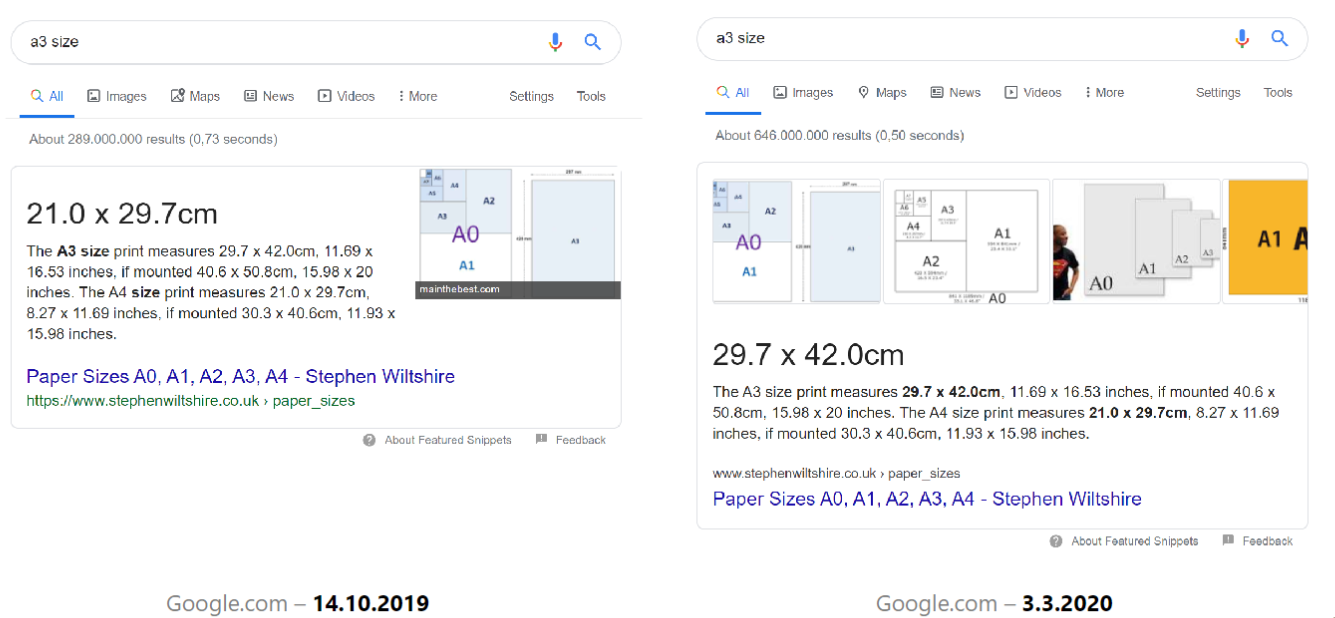
\includegraphics[width=1\textwidth]{assets/pics/google-ir.png}  
    \end{figure}
\end{frame}


\frametitle{Alur Pemeringkatan Teks Klasik}
\begin{frame}
    \begin{figure}
        \centering
        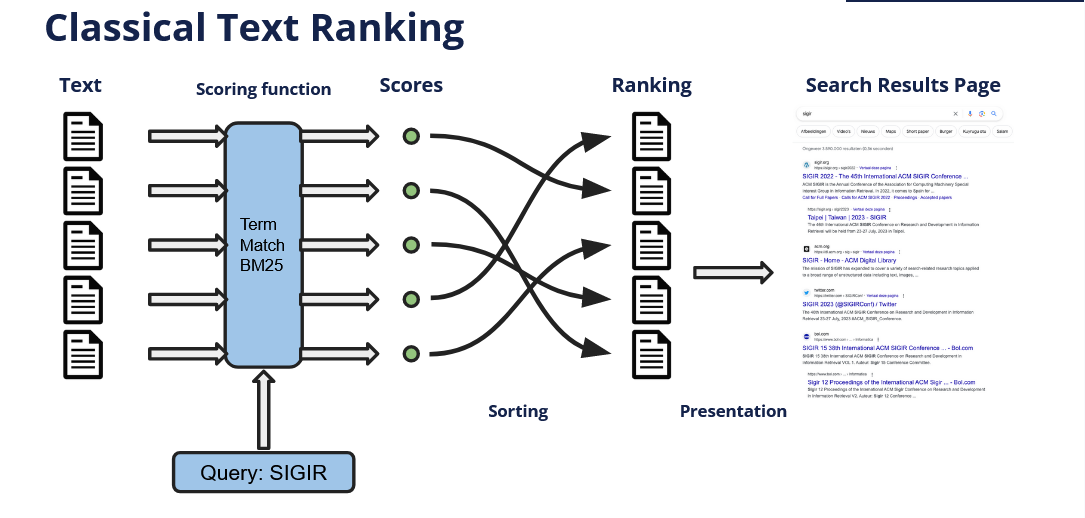
\includegraphics[width=1\textwidth]{assets/pics/classical-IR.png}
    \end{figure}
\end{frame}

\begin{frame}{\f{Vocabulary Mismatch}}
    \begin{enumerate}
        \item Pemeringkatan teks dengan kecocokan kata antara kueri dan teks memiliki kelemahan, yaitu sistem tidak dapat mengambil teks yang relevan bila kueri dan teks memiliki kata yang berbeda.
        \item Sebagai contoh, untuk kueri \code{apa makanan ternenak di Indonesia}, teks dengan kalimat \code{hidangan terlezat di nusantara adalah rendang} tentunya akan mendapatkan skor yang rendah karena tidak memiliki kata yang sama dengan kueri.
        \item Dengan memanfaatkan data tambahan seperti log atau jumlah klik (pada web) dari teks, model \f{machine learning} dapat digunakan untuk memeringkatkan teks.
    \end{enumerate}
\end{frame}

\begin{frame}
\frametitle{Alur Pemeringkatan Teks dengan \f{Machine Learning}}
    \begin{figure}
        \centering
        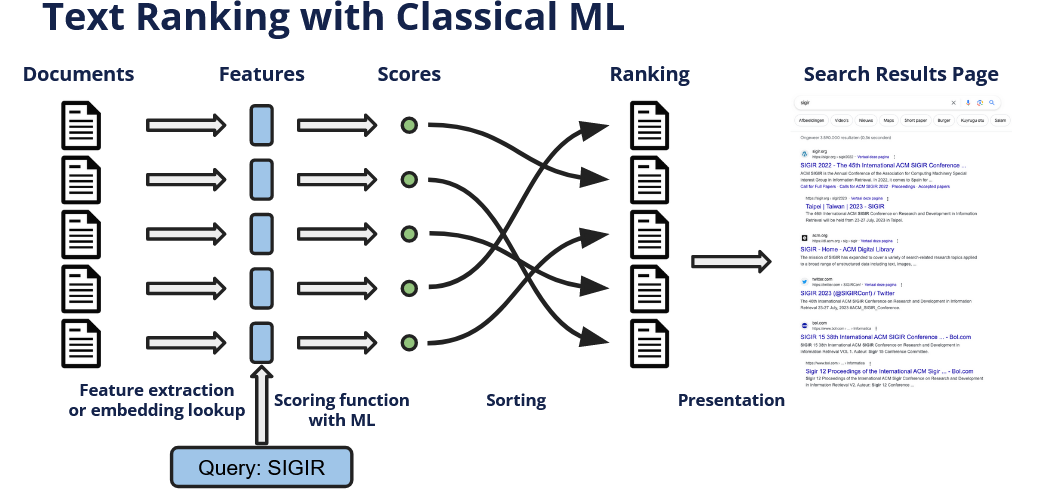
\includegraphics[width=1\textwidth]{assets/pics/LTR-IR.png}
    \end{figure}
\end{frame}

\begin{frame}
    \frametitle{Pemeringkatan Teks dengan \f{Machine Learning}}
    \begin{enumerate}
        \item Kekurangan penggunaan \f{machine learning} untuk pemeringkatan adalah jumlah fitur tambahan yang dibutuhkan cukup banyak untuk mengimbangi kekurangan dari BM25, dan fitur tersebut biasanya dibuat secara manual \citep{textrankingsurvey}.
        \item Batasan yang dialami model \f{machine learning} pada era \f{learning to rank}, diatasi dengan menggunakan \f{deep learning}.
    \end{enumerate}

\end{frame}

\begin{frame}
    \frametitle{Alur Pemeringkatan Teks dengan \f{Deep Learning}}
    \begin{figure}
        \centering
        \includegraphics[width=1\textwidth]{assets/pics/deep-IR.png}
    \end{figure}
\end{frame}

\begin{frame}

    
\end{frame}

\begin{frame}
\frametitle{Rumusan Masalah}

\begin{enumerate}
	\item Bagaimana pengaplikasian model BERT untuk pemeringkatan teks berbahasa Indonesia?
	\item Bagaimana kinerja model BERT pada setiap \f{dataset} yang digunakan bila dibandingkan dengan model \f{baseline} BM25?
\end{enumerate}

\end{frame}

\begin{frame}
    \frametitle{Tujuan Penelitian}
    \begin{enumerate}
        \item Membangun dan melatih kembali \f{(fine tuning)} model BERT untuk pemeringkatan teks berbahasa Indonesia.
        \item Membandingkan kinerja model BERT pada setiap \f{dataset} yang digunakan bila dibandingkan dengan model \f{baseline} BM25.
    \end{enumerate}
\end{frame}

\begin{frame}
    \frametitle{Batasan Masalah}
    \begin{enumerate}
    \item \f{Dataset} yang digunakan untuk melatih kembali (\f{fine tuning}) model BERT adalah \f{dataset} Mmarco \f{train set} bahasa Indonesia \citep{mmarco}.
	\item \f{Dataset} yang digunakan untuk mengukur performa model adalah \f{dataset} Mmarco \f{dev set} bahasa Indonesia \citep{mmarco} untuk \f{in-domain test} serta MrTyDi \f{dev set} bahasa Indonesia \citep{mrtydi}, dan Miracl \f{dev set} bahasa Indonesia \citep{miracl} untuk \f{out-of-domain test}.
	\item Kinerja model diamati dengan metrik \f{recriprocal rank} (RR), \f{recall} (R), dan \f{normalized discounted cumulative gain} (NDCG).
    \end{enumerate}
\end{frame}
    
\section{Pemeringkatan Teks}

\begin{frame}
\frametitle{Pemeringkatan Teks 1}

    \begin{block}{Tugas Pemeringkatan Teks}
        Diberikan kueri $q$ dan himpunan teks terbatas $\mathcal{D}= \{d_1, d_2, ..., d_n\}$, keluaran yang diinginkan dari permasalahan ini adalah barisan teks $D_k = (d_{i_1}, d_{i_2}, ..., d_{i_k})$ yang merupakan $k$ teks yang paling relevan dengan kueri $q$.
    \end{block}

    \noindent\f{Dataset} Uji pada masalah pemeringkatan teks terdiri dari tiga \f{file}, yaitu \f{file} kueri, \f{file} korpus dan \f{file judgements}.
\end{frame}


\begin{frame}
    \frametitle{Pemeringkatan Teks 2}
    \begin{table}[!ht]
        \centering
        \label{tab:contoh-file-korpus}
        \caption{\f{File} korpus}
        \begin{tabular}{|l|l|p{0.3\textwidth}|}
            \hline
            \textbf{\_id}    & \textbf{title}             & \textbf{text}                                                                                                 \\ \hline
            1342516\#1  & Colobothea biguttata & Larva kumbang ini biasanya mengebor ke dalam kayu dan dapat menyebabkan kerusakan $\dots$ \\ \hline
            1342517\#0  & Ichthyodes rufipes  & Ichthyodes rufipes adalah spesies kumbang tanduk panjang yang berasal dari famili Cerambycidae. Spesies ini $\dots$ \\ \hline
        \end{tabular}
    \end{table}
\end{frame}


\begin{frame}
\frametitle{Pemeringkatan Teks 3}

    \begin{table}[!ht]
        \centering
        \caption{\f{File} kueri}
        \label{tab:query-file-example}
        \begin{tabular}{|l|p{0.3\textwidth}|}
            \hline
            \textbf{\_id} & \textbf{text}                                                                 \\ \hline
            3             & Dimana James Hepburn meninggal?                                              \\ \hline
            4             & Dimana Jamie Richard Vardy lahir?                                            \\ \hline
            11            & berapakah luas pulau Flores?                                                 \\ \hline
            17            & Siapakah yang menulis Candy Candy?                                           \\ \hline
            19            & Apakah karya tulis Irma Hardisurya yang pertama?                              \\ \hline
        \end{tabular}
    \end{table}
\end{frame}


\begin{frame}
\frametitle{Pemeringkatan Teks 4}

    \begin{table}[!ht]
        \centering
        \caption{\f{File judgements}}
        \label{tab:judgements-file-example}
        \begin{tabular}{|l|l|l|}
            \hline
            \textbf{query-id} & \textbf{corpus-id} & \textbf{score} \\ \hline
            3                 & 115796\#6          & 1              \\ \hline
            3                 & 77689\#48          & 1              \\ \hline
            4                 & 1852373\#0         & 1              \\ \hline
        \end{tabular}
    \end{table}
\end{frame}

\section{Metrik Evaluasi}

\begin{frame}
    \frametitle{\f{Recall} dan Presisi}
    \begin{columns}
        \column{0.7\textwidth}
        \begin{align*}
            \text{recall}(q, D_k)\text{@k} &= \frac{\sum_{d \in D_k} \text{rel}(q, d)}{\sum_{d \in \mathcal{D}} \text{rel}(q, d)} \in [0, 1], \\ 
            \text{precision}(q, D_k)\text{@k} &= \frac{\sum_{d \in D_k} \text{rel}(q, d)}{|D_k|} \in [0, 1], \\
            \text{rel}(q, d) &= \begin{cases} 
            1 & \text{jika } r > 1 \\
            0 & \text{jika } r = 0
            \end{cases}.
        \end{align*}

        \column{0.3\textwidth}
        \begin{itemize}
            \item $q$: kueri,
            \item $D_k$: barisan $k$ teks yang dipilih oleh sistem,
            \item $r$: nilai relevansi antara kueri $q$ dengan teks $d$ dari \f{file} judgements.
        \end{itemize}
    \end{columns}
\end{frame}

\begin{frame}
    \frametitle{\f{Recall} dan Presisi}
    \begin{figure}[!ht]
        \centering
        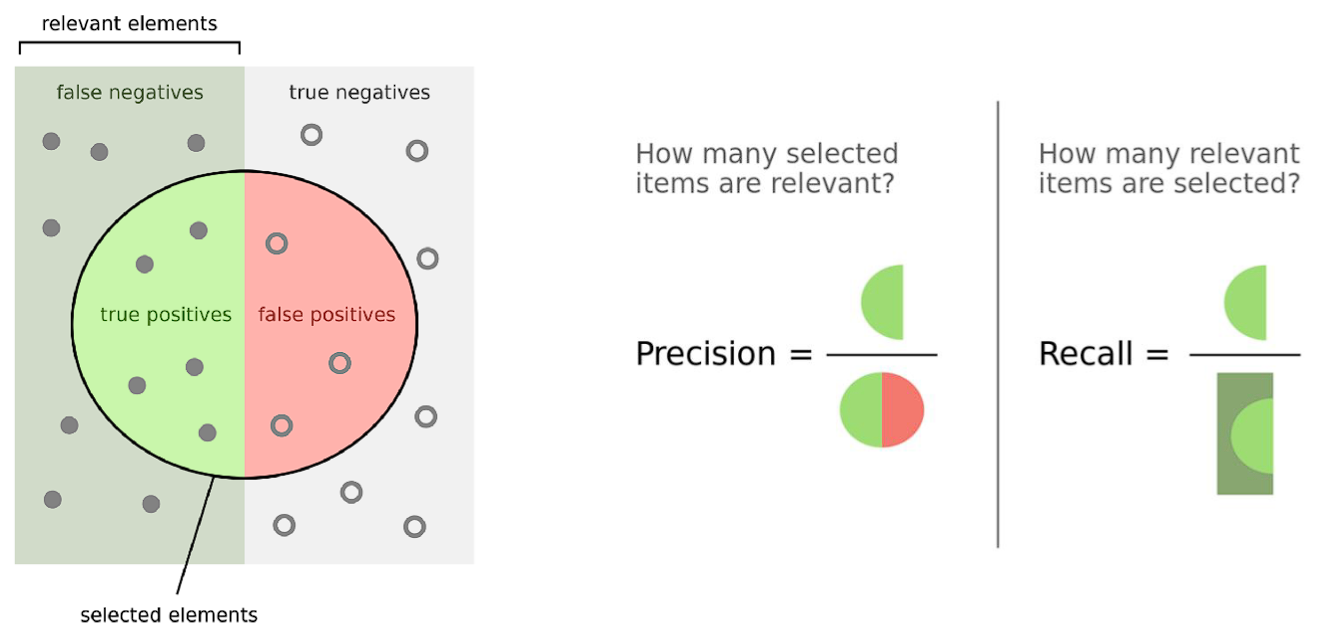
\includegraphics[width=1\textwidth]{assets/pics/recall-presisi.png}
        \caption{Ilustrasi \f{recall} dan presisi.}
        \label{fig:recall-precision}
    \end{figure}
\end{frame}

\begin{frame}
    \frametitle{\f{Reciprocal Rank}}
    Metrik lainnya yang sering digunakan untuk mengukur performa sistem pemeringkatan adalah \f{reciprocal rank} (RR). Metrik RR menitikberatkan pada peringkat dari teks relevan pertama dengan kueri $q$.

        \begin{align*}
            \text{RR}(q, D_k)\text{@k} &= \begin{cases}
                \frac{1}{\text{FirstRank}(q, D_k)} & \text{jika } \exists d \in D_k \text{ dengan } \text{rel}(q, d) = 1 \\        
                0 & \text{jika } \forall d \in D_k, \text{ rel}(q, d) = 0 \\
                \end{cases},
        \end{align*}
        
        \begin{itemize}
            \item $q$: kueri,
            \item $D_k$: barisan $k$ teks yang dipilih oleh sistem,
            \item $r$: nilai relevansi antara kueri $q$ dengan teks $d$ dari \f{file} judgements.
            \item $ \text{FirstRank}(q,D_k)$: $\text{posisi teks relevan pertama } d\in D_k \text{ dengan } \text{rel}(q, d) = 1. $
        \end{itemize}
\end{frame}


\begin{frame}
    \frametitle{\f{Reciprocal Rank}}
    \begin{figure}[!ht]
        \centering
        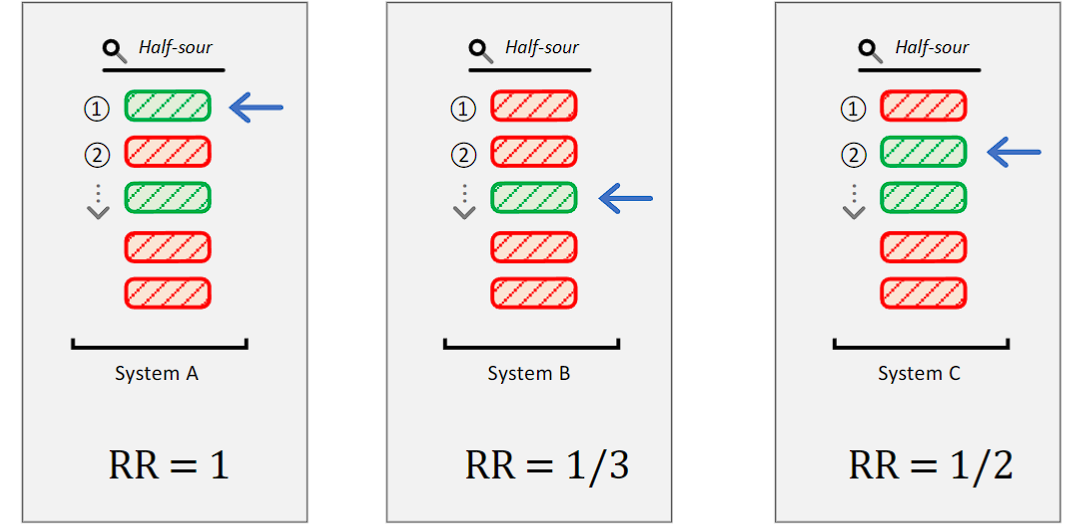
\includegraphics[width=1\textwidth]{assets/pics/rr.png}
        \caption{Ilustrasi \f{reciprocal rank}.}
        \label{fig:reciprocal-rank}
    \end{figure}
\end{frame}

\begin{frame}
    \frametitle{\f{Normalized Discounted Cumulative Gain}}
    \f{Normalized Discounted Cumulative Gain} (NDCG) adalah metrik yang umumnya digunakan untuk mengukur kualitas dari pencarian situs web. Tidak seperti metrik yang telah disebutkan sebelumnya, nDCG dirancang untuk suatu $r$ yang tak biner.
    \begin{flalign*}
        \text{nDCG}(q, D_k)\text{@k} &= \frac{\text{DCG}(q, D_k)\text{@k}}{\text{DCG}(q, D_k^{\text{ideal}})\text{@k}} \in [0, 1], && \\
        \text{DCG}(q, D_k)\text{@k} &= \sum_{d \in D_k} \frac{2^{\text{rel}(q, d)} - 1}{\log_2(\text{rank}(d, D_k) + 1)}, && \\
        \text{rank}(d,D_k) &= \text{Posisi } d \text{ dalam } D_k, && \\
        \text{rel}(q, d) &= r. &&
    \end{flalign*}  

\end{frame}

\begin{frame}
    \frametitle{\f{Normalized Discounted Cumulative Gain}}
    \begin{figure}[!ht]
        \centering
        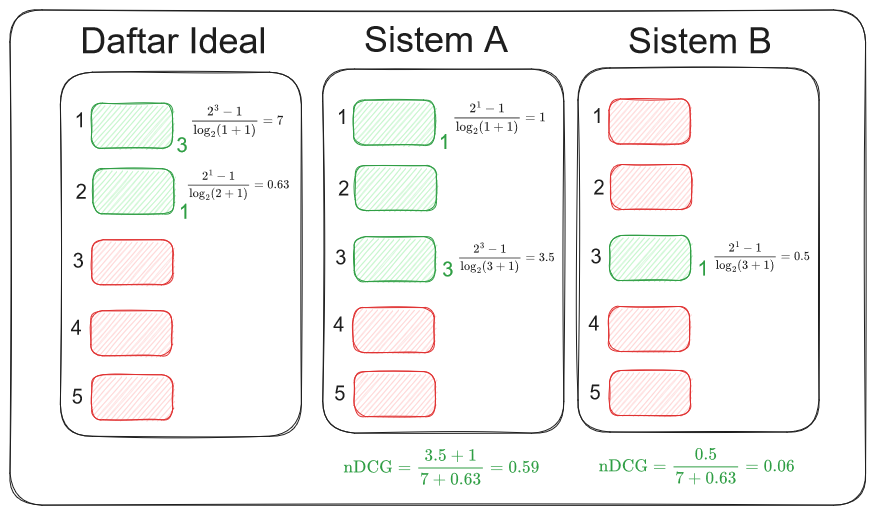
\includegraphics[width=1\textwidth]{assets/pics/contohnDCG.png}
        \caption{Ilustrasi \f{normalized discounted cumulative gain}.}
        \label{fig:ndcg}
    \end{figure}
\end{frame}

\section{Pemeringkatan Teks Dengan Statistik}

\begin{frame}
    \frametitle{{Pemeringkatan Teks Dengan Statistik}}

    \begin{enumerate}
        \item Untuk mengambil $k$ teks dari kumpulan $\mathcal{D}$, kita menggunakan fungsi skor $\text{score}(q, d, \mathcal{D})$ untuk mengukur relevansi antara kueri $q$ dan teks $d$. Dengan mencari skor antara $q$ dan semua teks pada $\mathcal{D}$, kita dapat memilih barisan teks $D_k = (d_{i_1}, d_{i_2},\dots, d_{i_k})$ dengan $k$ teks memiliki skor tertinggi.
        \item Salah satu fungsi skor mudah dan sering digunakan adalah TF-IDF dan BM25. Fungsi skor ini menghitung skor antara kueri $q$ dan teks $d$ dengan informasi dari kata yang ada pada $q$ dan $d$.
    \end{enumerate}
\end{frame}

\begin{frame}
    \frametitle{TF-IDF}
    \begin{itemize}
        \item \f{term frequency}: $\text{tf}(t, d) = \frac{\text{Count}(t, d)}{|d|}$,
        \item \f {document frequency}: $\text{df}(t, \mathcal{D}) = \text{jumlah teks pada } \mathcal{D} \text{ yang mengandung kata } t$. 
        \item \f{inverse document frequency}: $\text{idf}(t, \mathcal{D}) = \begin{cases}
            \log_2\left(\frac{|\mathcal{D}|}{\text{df}(t, \mathcal{D})}\right) & \text{jika } \text{df}(t, \mathcal{D}) > 0 \\
            0 & \text{jika } \text{df}(t, \mathcal{D}) = 0
        \end{cases}$.
        \item $\text{TF-IDF}(t, d, \mathcal{D}) = \text{tf}(t, d) \times \text{idf}(t, \mathcal{D})$.
    \end{itemize}

    \begin{figure}[!ht]
        \centering
        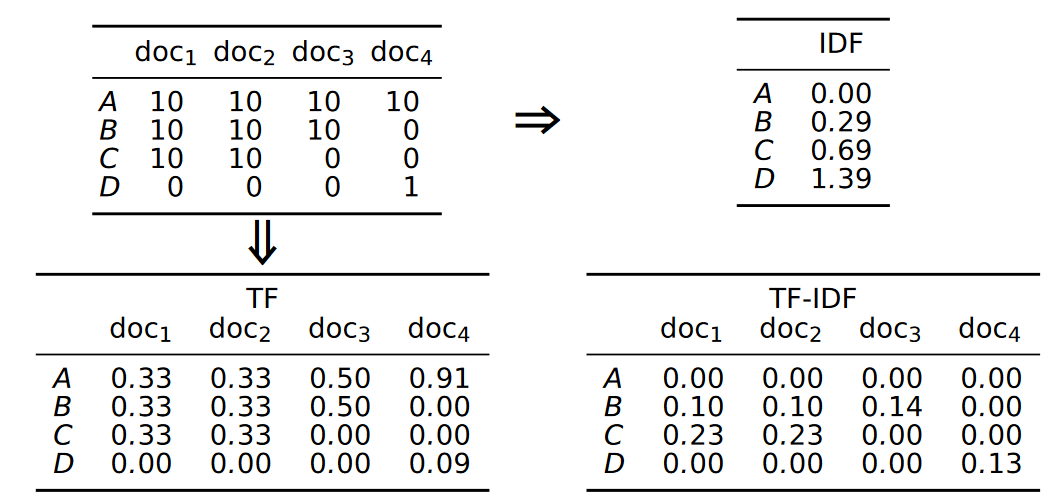
\includegraphics[width=1\textwidth]{assets/pics/tf-idf-matriks.png}
    \end{figure}
\end{frame}

\begin{frame}
    \frametitle{Nilai IDF}
    \begin{figure}[!ht]
        \centering
        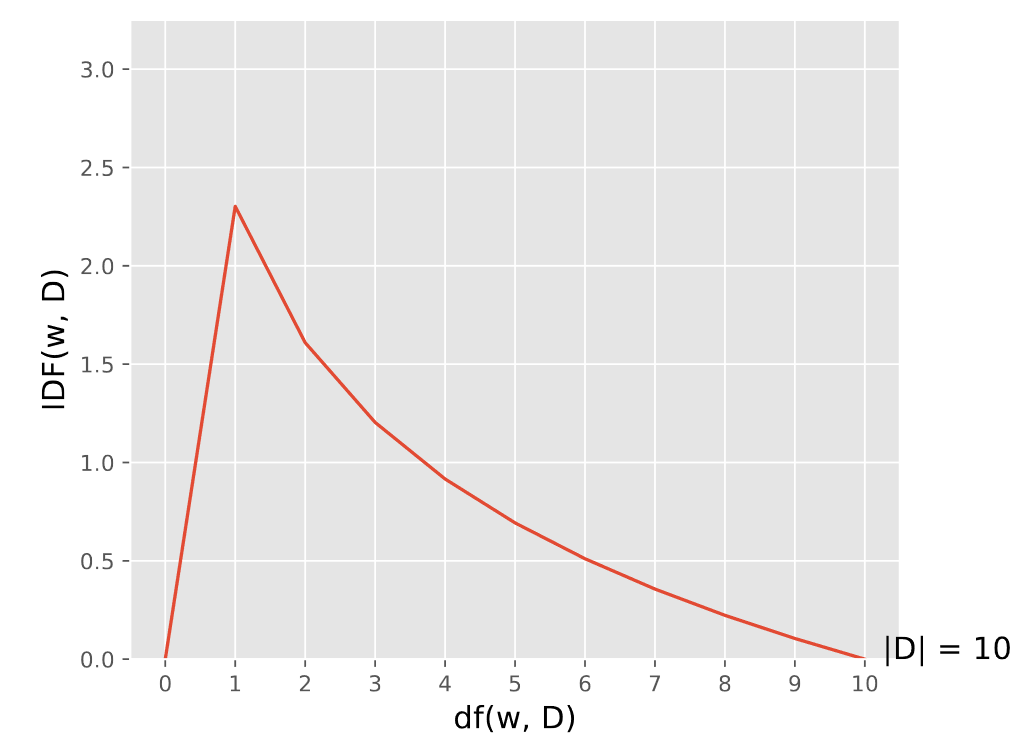
\includegraphics[width=1\textwidth]{assets/pics/idf-graph.png}
        \end{figure}
\end{frame}

\begin{frame}
    \frametitle{Score}

    $$\text{score}(q,d,\mathcal{D}) = \sum_{t \in T_q \cap T_d} \text{TF-IDF}(t, d, \mathcal{D})$$
    \begin{flalign*}
        T_q &= \{t_1, t_2, \dots, t_{L_1}\} = \text{kumpulan kata pada } q, && \\
        T_d &= \{t_1, t_2, \dots, t_{L_2}\} = \text{kumpulan kata pada } d. &&
    \end{flalign*}
\end{frame}

\begin{frame}
    \frametitle{BM25}

    \begin{block}{\f{Smoothed} IDF}
        $$
        \text{idf}_{\text{BM25}}(t, \mathcal{D}) = \log\left(1+\frac{|\mathcal{D}| - \text{df}(t, \mathcal{D}) + 0.5}{\text{df}(t, \mathcal{D}) + 0.5}\right)
        $$
    \end{block}

    \begin{block}{Score BM25 Pengganti tf}
        $$
        \text{score}_{\text{BM25}}(t,d) = \frac{\text{tf}(t, d) \times (k_1 + 1)}{\text{tf}(t, d) + k_1 \times (1 - b + b \times \frac{|d|}{\text{avgdl}})}
        $$
    \end{block}

    \begin{block}{BM25}
        $$
        \text{BM25}(t, d, \mathcal{D}) = \text{idf}_{\text{BM25}}(t, \mathcal{D}) \times \text{score}_{\text{BM25}}(q,d,\mathcal{D})
        $$
    \end{block}
    \cite{BM25ori}
\end{frame}

\section{Mekanisme \f{Attention}, \f{Transformer} dan BERT}

\begin{frame}
    \frametitle{Mekanisme \f{Attention}}
\end{frame}

\begin{frame}
    \frametitle{\f{Soft Attention}}
\end{frame}

\begin{frame}
    \frametitle{\f{Attention} Parametrik}
\end{frame}

\begin{frame}
    \frametitle{Transformer}
\end{frame}

\section{}

\begin{frame}
    
\end{frame}


\begin{frame}[allowframebreaks]
    \frametitle{Daftar Pustaka}
    \bibliography{references}
\end{frame}

\end{document}